\myNewSlide
\section*{Scenario}\normalsize
\begin{enumerate}
    \item A (presumably evil) competing lab scoops you by publishing a tree, $T_1$, for your favorite group of organisms.
    \item You have just collected a new dataset for the group, and your ML estimate of the best tree, $T_2$, differ's from $T_1$.
    \item A KH Test shows that your data {\bf significantly} prefer $T_2$ over $T_1$.
    \item You write a (presumably scathing) response article.
\end{enumerate}
Should a {\em Systematic Biology} publish your response?

\myNewSlide\large
\section*{What if start out with only one hypothesized tree, and we want to compare it to the ML tree?}
The KH Test is {\bf NOT} appropriate in this context \citep[see][for discussion of this point]{GoldmanAR2000}
    
{\bf Multiple Comparisons}: lots of trees increases the variance of $\delta(\hat{T},T_1 \mid X)$\\

{\bf Selection bias}: Picking the ML tree to serve as one of the hypotheses invalidates the centering procedure of the KH test.

\myNewSlide
\section*{Using the ML tree in your test introduces selection bias}
Even when the $H_0$ is true, we do not expect $2\left[\ln L(\hat{T}) - \ln L(T_1)\right]= 0$

Imagine a competition in which a large number of equally skilled people compete, and you compare the score of one competitor against the highest scorer.

\myNewSlide
\begin{picture}(500,0)(0,0)
      \put(-10,15){Experiment: 70 people each flip a fair coin 100 times and}
      \put(0,-20){count \# heads.}
      \put(100,-55){$h_1 - h_2$}
      %\put(400,-55){$\max(h) - h_1$}
      \put(-30,-250){\makebox(0,0)[l]{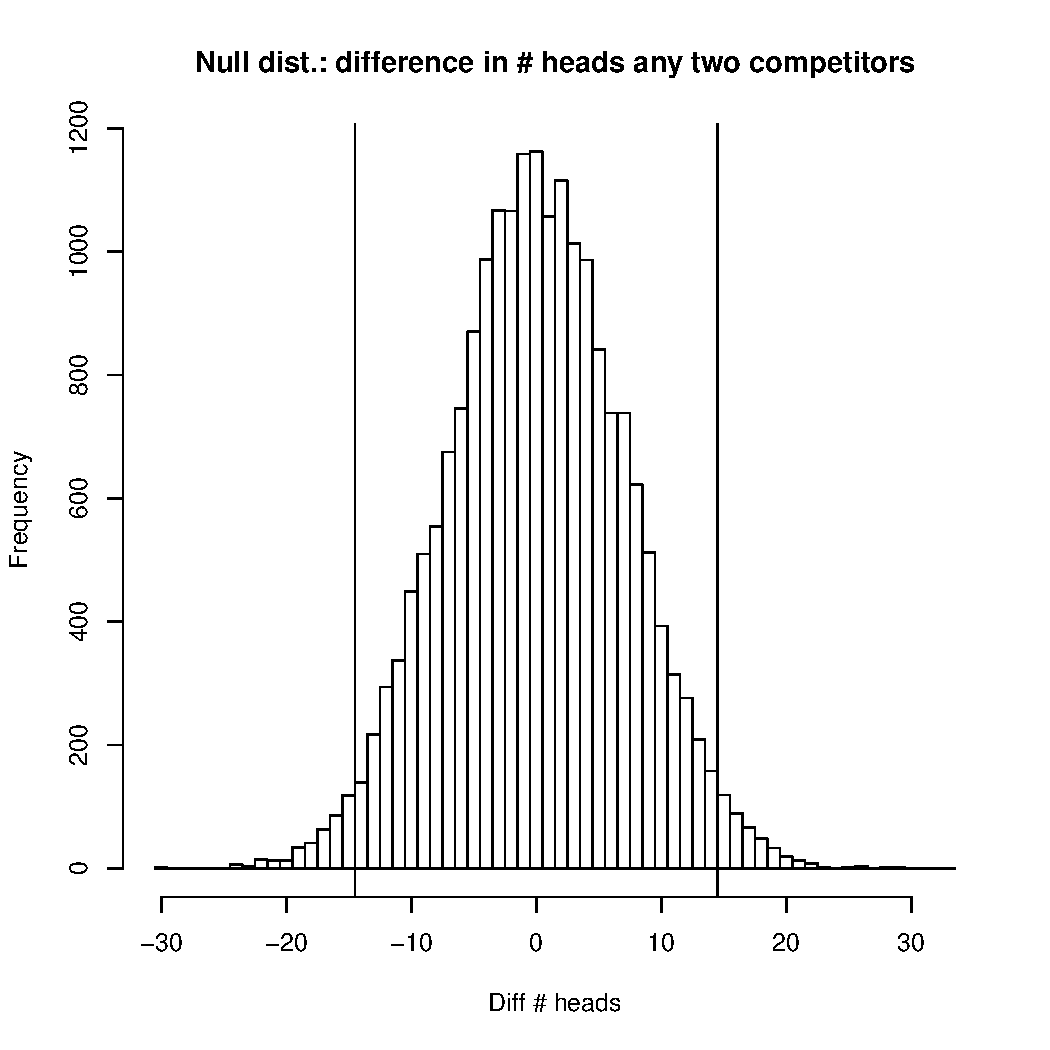
\includegraphics[scale=.75]{../scripts/cfc_diff_a_priori.pdf}}}
\end{picture}

\myNewSlide
\begin{picture}(500,0)(0,0)
      \put(-10,15){Experiment: 70 people each flip a fair coin 100 times and}
      \put(0,-20){count \# heads.}
      \put(100,-55){$h_1 - h_2$}
      \put(400,-55){$\max(h) - h_1$}
      \put(-30,-250){\makebox(0,0)[l]{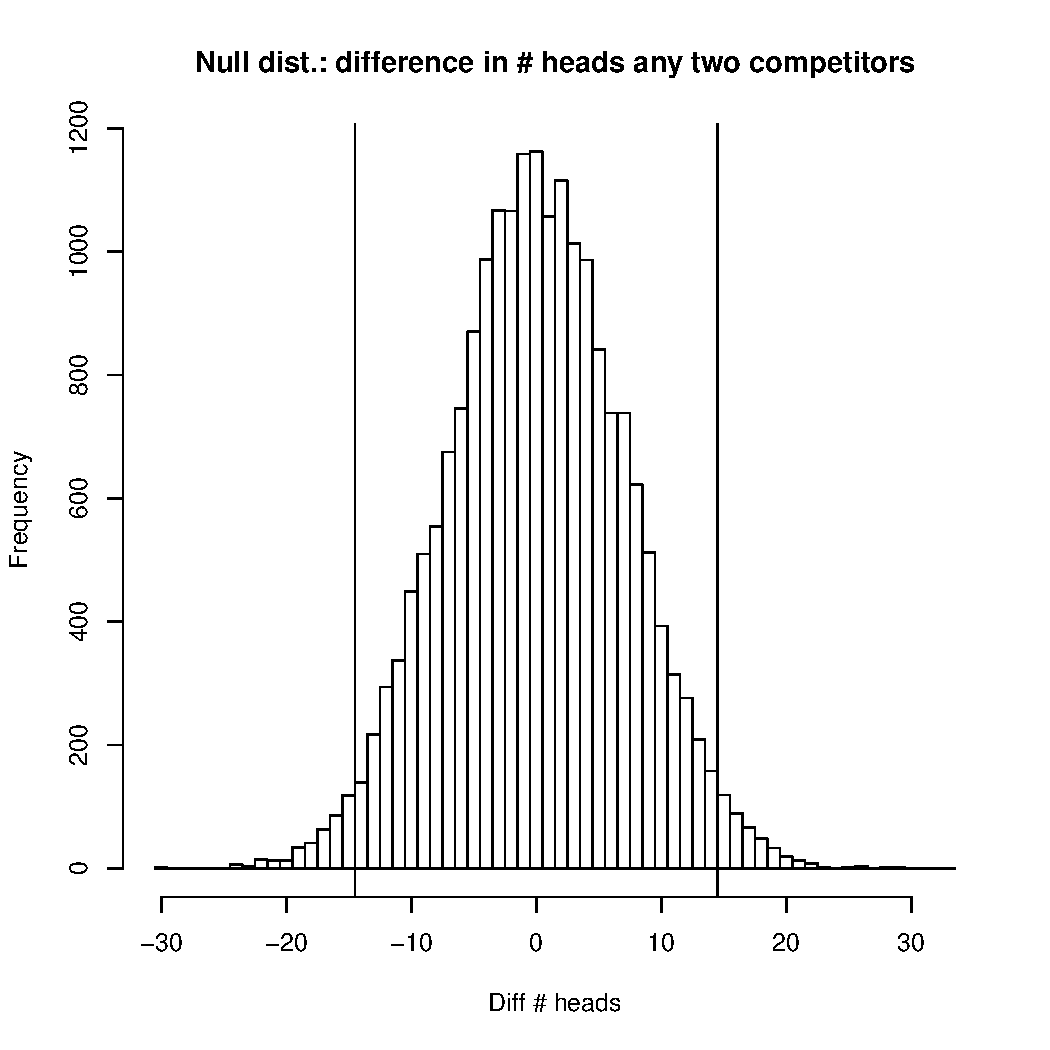
\includegraphics[scale=.75]{../scripts/cfc_diff_a_priori.pdf}}}
      \put(320,-250){\makebox(0,0)[l]{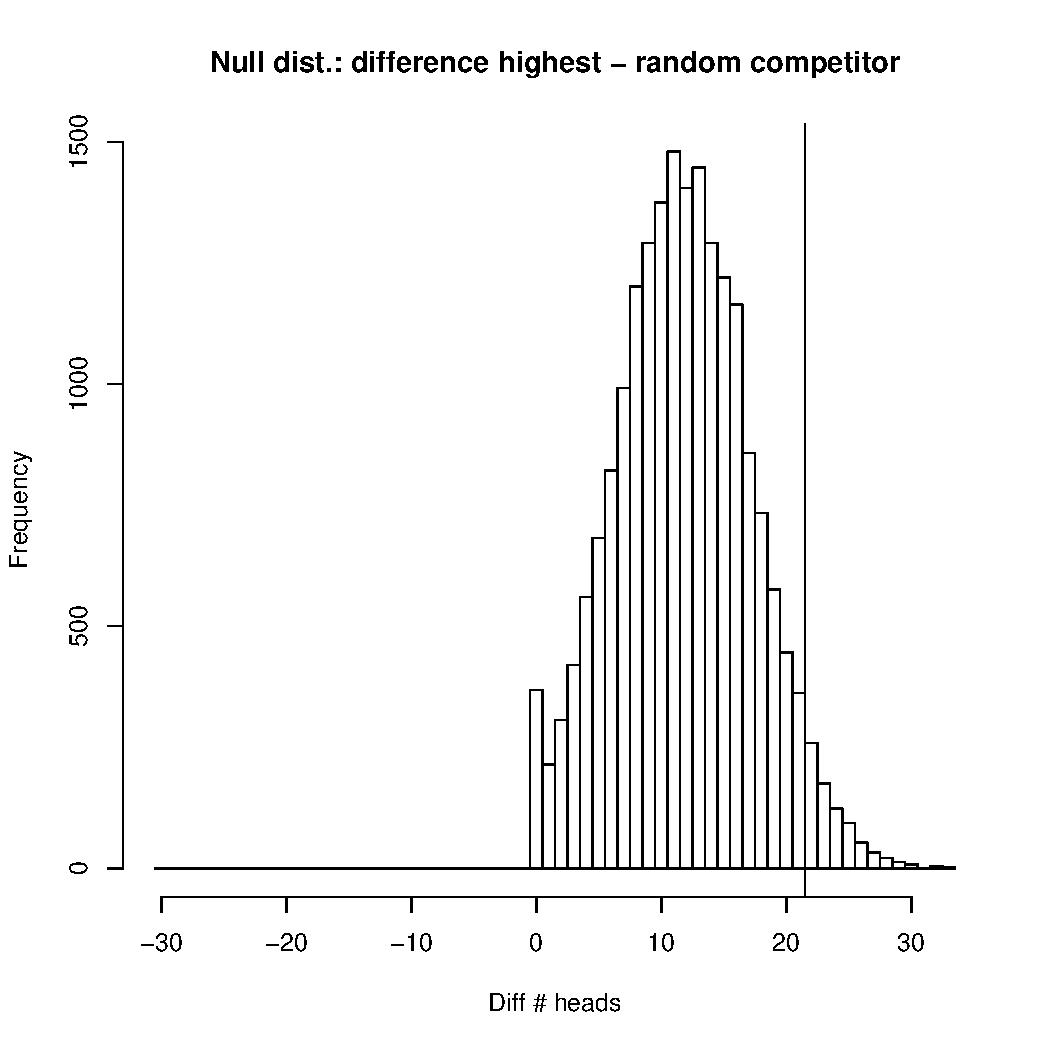
\includegraphics[scale=.75]{../scripts/cfc_diff_best_v_one.pdf}}}
\end{picture}


\myNewSlide 
\section*{Shimodaira and Hasegawa proposed the SH test which deals the ``selection bias'' introduced by using the ML tree in your test}
Requires {\bf set of candidate trees} - these {\bf must not} depend on the dataset to be analyzed.

$H_0$: each tree in the candidate set is as good as the other trees.

The test makes worst-case assumptions - it {\bf is conservative}.

AU test is less conservative (still needs a candidate set)

